% Header {{{
% vim: ft=tex:fdm=marker:cc=:
\documentclass[a4paper]{article}

% Plugins {{{
    \usepackage[T1]{fontenc}
    \usepackage[utf8]{inputenc}
    \usepackage[icelandic]{babel}

    \usepackage{url}
    % Graphics
        \usepackage{graphicx}
        \graphicspath{{visualisation/graphics/}}
        \usepackage{subfig}
    \usepackage{amsmath}
% }}}

\title{Krónan eða Evran fyrir Ísland?}
\author{Árni Dagur}
% }}}
\begin{document}
\maketitle

\section{Inngangur}

Lengi vel hefur innganga Íslands inn í Evrusvæðið verið umræðumál hér á landi, og magnaðist sú umræða mjög eftir hrunið mikla árið 2008. Hægt er að móta rök með og á móti upptöku hennar, og er hægt að finna fræðimenn sem tala fyrir hendi beggja hliða. Í þessu riti verður farið yfir þessi rök og í lok þess lýsir höfundur sinni persónulegri skoðun.

% Í viðtali við \textit{The Guardian} lýsti háttsettur Íslenskur embættismaður sem ekki vildi láta nafns síns getið vantrausti sínu til krónunnar. \textit{''The Krona is dead. We need a new currency. The only serious option is the euro.''} sagði hann.\cite{traynor_2009}

\section{Rök með}

\subsection{Aukinn stöðugleiki gjaldmiðils}
\begin{figure} %{{{Volatility.png
    \centerline{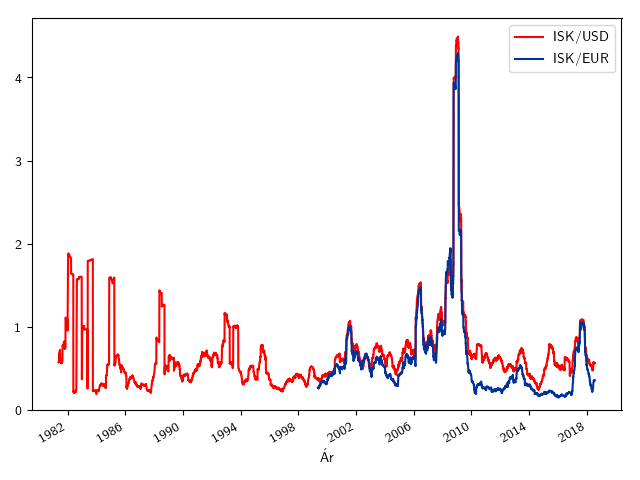
\includegraphics{volatility.png}}
    \caption{Staðalfrávik prósentubreytingar með 90 daga rúllandi ramma. Gögn koma frá Seðlabanka Íslands.}
    \label{fig:volatility}
\end{figure} %}}}

Árið 2008 var stöðugleiki krónunnar miðað við önnur lönd rannsakaður af René Kallestrup, hagfræðing Seðlabanka Íslands. Niðurstaða þessarar rannsóknar leiddi í ljós að óstöðugleiki íslensku Krónunnar er einn þeirra hæstu miðað við aðra gjaldmiðla þróuðu ríkjanna. Þó er óstöðugleiki Íslensku krónunnar lægri en hjá gjaldmiðlum flestra þróunarríkja. Stöðugleiki Evrunnar er aftur á móti þó nokkuð meiri – svipaður Bandaríkjadalnum.\cite{icb_volatility_2008}

Á Mynd~\ref{fig:volatility} sést óstöðugleiki Krónunnar miðað við Bandaríkjadalinn og Evruna vel. Hann er skilgreindur sem staðalfrávik prósentumuns á 90 daga rúllandi ramma.


\subsection{Minni þörf á að geyma varaforða erlenda gjaldmiðla}

Vegna þess eins að Evrusvæðið hafi verið stofnað hefur þörf Seðlabanka Íslands til þess að geyma erlenda gjaldmiðla minnkað. Í staðinn fyrir marga sjóði fyrir hvert Evrópuríki sem Ísland gerir viðskipti við (þýsk Mörk, franskir Frankar, spænskir Pesóar, etc) getur hann haldið einn Evrusjóð fyrir öll ríki Evrusvæðisins.

Við upptöku Evrunnar gæti Ísland minnkað forða sinn á gjaldmiðlinum enn frekar\cite{saga_evropusamrunans}, en árið 2017 voru Evrur 30\% forðans.\cite{icb_annual_2017}

\subsection{Aukin viðskipti við Evrusvæðið}

Árið 2004 gerði Þórarinn G. Pétursson, sem nú er aðalhagfræðingur Seðlabanka Íslands, rannsókn í samvinnu við breskan hagfræðing þar sem reynt var að leggja tölu á kosti þess að ganga inn í Evrusvæðið. Notast var við svokallað \textit{Gravity Model of Trade} eða þyngdaraflsmódel alþjóðaviðskipta til að leggja mat á áhrif semeiginlegs gjaldmiðils, og gjaldmiðlaóstöðuleika á alþjóðleg viðskipti, líkt og lýst var af Rose et al.\cite{rose2000} Nafnið má rekja til þess að aðaljafnan sem lýsir módeli þessu líkist mjög þyngdarkraftslögmáli Newtons, eins og sést hér fyrir neðan.

\[F_{ij} = G\frac{M_{i}M_{j}}{r^{2}} \qquad X_{ij} = G\frac{Y_{i}Y_{j}}{D_{ij}}\eta_{ij}\]

Fyrsta jafnan er auðvitað jafna þyngdarkraftslögmáls Newtons; \(G\) er fasti, \(M_{i}\) og \(M_{j}\) merkir massa hlutanna tveggja, \(r\) fjarlægðina, og \(F_{ij}\) þyngarkraftinn á milli þeirra. Seinni jafnan er jafna þyngdarkraftsmódels alþjóðaviðskipta; hér merkir \(X_{ij}\) útflutning \(i\) til \(j\), \(G\) er einnig fasti, \(Y_{i}\) og \(Y_{j}\) eru svokallaðir ``efnahagslegir massar'' jafnir þjóðarframleiðslu, \(D_{ij}\) er sá viðskiptakostnaður sem við erum að reyna að mæla áhrifin af, og loks et \(\eta_{ij}\) fráviksfasti. Hægt er að nálgast \(X_{ij}\) með venjulegri aðferð minnstu kvaðrata. Logrinn er þá tekin af báðum hliðum, og fáum við þá:

\[\ln(X_{ij}) = \beta_{0} + \beta_{1}\ln(Y_{i}) + \beta_{2}\ln(Y_{j}) - \beta_{3}\ln(D_{ij}) + \epsilon_{ij}\]

Þar sem \(\beta_{1}\), \(\beta_{2}\), og \(\beta_{3}\) eru jákvæðir fastar, og \(\epsilon_{ij}\) er frávikið. Takið eftir að \(G\) er hér partur af \(\beta_{0}\). Fastarnir \(\beta_{1}\), \(\beta_{2}\), og \(\beta_{3}\) eru svo valdir fyrir minnsta mögulega gildi \(\sum_{i}\sum_{j}\epsilon_{ij}^{2}\).\cite{gravity_powerpoint} Þeir komust að þeirri niðurstöðu að það megi búast við 60\% viðskiptaaukningu við það að ganga í Evrusvæðið. Helmingur þess gróða mætti rekja til þess eins að ganga í ESB, en hinn helminginn til upptöku Evrunnar. Ástæðan fyrir því má einmitt að mörgu leyti rekja til ofanlýstra punkta.\cite{icb_wp_26}

Í kennslubókinni \textit{Economics} sem er kennd í þessum áfanga er sú staðreynd að alþjóðaviðskipti gerir báða aðila betur af lýst sem ein af 10 grundvallarreglum hagfræðinnar.\cite{economics} Aukning nær 60 prósentustigum á alþjóðaviðskiptum við Evrusvæðið væri því mjög góð fyrir Ísland, sérstaklega þar sem stór hluti alþjóðaviðskipta Íslendinga eru nú þegar við Evrusvæðið.\cite{hvada_gjaldmidill}

\section{Rök á móti}

\subsection{Missir á eigin peningastefnu}

\subsubsection{Dæmið um Grikkland}

Í venjulegum kringumstæðum þar sem land hefur hefur fullt vald yfir gjaldmiðli sínum mun það bregðast við miklu atvinnuleysi með því að prenta meiri pening. Það lækkar virði gjaldmiðilsins og þar með hækkar ferðamannastraum, fjárfestingar, og gróða útflutningsgreina. Ef atvinnuleysi er lágt, aftur á móti, mun það prenta minni pening og þar með hækka kaupmátt og lækka verð á vörum. Þetta getur þó Grikkland ekki gert af því hvernig Evrusvæðið er sett upp. Þó að Grikkland stjórni sínum eigin ríkisfjármálum, stjórnar Seðlabanki Evrópusambandsins peningastefnu þess.\cite{vox_greece} Styrkur gjaldmiðils sem er tilvalinn fyrir Þýskaland, þar sem atvinnuleysi var 5.1\% árið 2014 er allt annar en styrkur gjaldmiðils sem er tilvalinn fyrir Grikkland, þar sem atvinnuleysi var 27.2\%.\cite{eurostat}

\subsubsection{Dæmið um Ísland}

Eftir hrunið mikla árið 2008 var Ísland í sambærilegri stöðu, en þó höfðum við stjórn á okkar peningastefnu. Sú staðreynd reyndist Íslendingum vel: Fall krónunnar leiddi til ófordæms áhuga erlendra ferðamanna á eyjunni sem ódýran áfangastað,\cite{worldfinance_2015} en ferðamennska til landsins er nú 320\% af því sem hún var árið 2006, fyrir hrunið.\cite{hagstofan_passengers} Útflutningsgreinar Íslands, sérstaklega fiskiðnaðurinn, sáu einnig stórar aukningar á tekjum sínum. Ísland er nú alþjóðlegt kennslubókardæmi um hvernig hrun gjaldmiðils getur leitt til hraðrar efnahagsbötnunar.\cite{worldfinance_2015}

Ef Ísland hefði verið með Evruna árin eftir hrunið mikla 2018, væri svo sannarlega hægt beita þeim rökum sem fram komu fyrir ofan að Ísland væri nú í sömu stöðu og Grikkland.

\subsection{Skortur á sameiginlegri fjármálastefnu}

Eins og Berger et al. lýstu í ritgerð sinni \textit{''Revisiting the Economic Case for Fiscal Union in the Euro Area''} er nokkur hætta falin í því að deila sameiginlegri peningastefnu en ekki fjármálastefnu.

Ef Evrusvæðið væri eins og önnur svæði með sameiginlegan gjaldmiðil, til dæmis fylki Bandaríkjanna, myndu meðlimir þess takast á við hagfræðilega erfiðleika saman. Miðstjórnin hefði tækin til að færa til pening og létta á svæðum í sérstökum efnahagslegum erfiðleikum. Líkt og höfundarnir segja hefur samvinna á þessu sviði vissulega aukist á síðastliðnum árum, en þó komi hún ekki í stað semeiginlegrar fjármálastefnu.\cite{fiscal_union}

Aukin fjárhagslegur agi væri einnig kostur við sameiginlega fjármálastefnu. Meginástæðan á bak við skuldakreppuna í Grikklandi er sú að eftir inngöngu Grikklands í Evrópusambandið lækkuðu vextirnir sem fjárfestar voru tilbúnir að lána ríkinu á verulega. Vextirnir á Grískum 10 ára ríkisskuldabréfum fóru frá um 25\% árið 1992 til um 5\% árið 2001, eftir upptöku Evrunnar. Fjárfestar héldu að Grikkland væri ei lengur hættuleg fjárfesting, og að ef til þess kæmi myndi önnur Evruríki líkt og Þýskaland og Frakkland veita því aðstoð. Þessi aukni aðgangur að ódýru fjármagni leiddi til þess að Grikkland fékk meira lánað en það gat borgað til baka; árið 2015 voru skuldir ríkisins 172\% af heildarframleiðslu. Við hrunið 2008, þegar lánin gufuðu upp, hrundi svo efnahagur Grikklands.\cite{vox_greece}

Annað vandamál Grikklands felst í því að skattasöfnun ríkisins er hlægilega lág miðað við önnur Evrópuríki; staðfestar skattaskuldir miðað við heildarsöfnun var 89,5\% árið 2010. Til samanburðar var tala Þýskalands sama ár 1,4\%, og tala Frakklands 6,8\%.\cite{oecd_greece_taxes}

Bæði þessi vandamál Grikklands höfðu líklega ekki orðið ef miðstjórn Evrópu, sem hefur reynst fjárhagslega agaðari heldur en sumar ríkisstjórnir meðlima sinna, til dæmis Grikklands, hefði umsjón um lán og skattasöfnun.

\section{Niðurstaða}

Því miður er ég ekki hagfræðingur, og treysti ég mér því ekki til þess að taka þessu stóru ákvörðun um upptöku Evrunnar fyrir hönd Íslendinga. Rök er þó greinilega hægt að færa fyrir báðum hliðum. Ætli ég myndi ekki fela fagfólki Seðlabankans þá ábyrgð að ákveða gjaldeyrisstefnu landsins.

\newpage
\bibliography{bibliography}
\bibliographystyle{plain}

\end{document}
